\section{Introduction}


Speech assisted computer interaction has increased in popularity over the past decade as speech recognition capability has improved and ubiquitous mobile computing devices such as tables, smartphones, in-home assistants, and vehicle entertainment systems integrate speech recognition into their core features. The SpeakQL project seeks to explore the possibility of moving the application of speech-based system interfaces from simple consumer-facing applications toward more technical areas such as data extraction from relational data stores.

SpeakQL 2.0 is an extension of previous research that implements a speech + touch interface to enable database querying using mobile devices with touchscreen interfaces. User feedback from usability studies performed on this system have motivated additional research, including the creation of a prototype dialect of SQL that, while retaining the expressive power and formality of SQL, creates a query dictation process that adheres to more natural speech patterns. This paper presents the motivation, justification, ongoing implementation, and ongoing evaluation of the SpeakQL dialect.


\section{Background}


\subsection{Motivation}

\subsubsection{Proliferation of Speech-Based Assistance Systems}

Speech-based assistance systems have become increasingly prevalent due to the growth of the mobile computing, internet of things, and smart device industries. With speech-based systems becoming more prevalent and accepted, we see opportunities to explore the possibility of applications that target a more technical user base. One such potential application is human-database interaction through spoken query dictation. This application has the potential to reduce barriers to employing data-driven decision making in organizations that often conduct critical operations in remote and/or austere conditions, or whos decision-making workers and analysts operate for long periods of time away from their computer workstations.

\subsubsection{Target Users}

The SpeakQL voice + touch query system was designed with input from the target user population: data analysts who require ad-hoc query capability while performing tasks in environments where they do not have immediate access to traditional computing equipment, and must rely on a mobile device. In prior SpeakQL work, conversations with practitioners revealed a need for SQL-knowleable analysts to access their data in ad-hoc ways while working in environments where standard keyboard-typed querying is not feasible. \cite{Shah2020}. In this paper, the authors identified on-the-go database administrators and data analysts, nurse informaticists, and individuals with motor disabilities as users who could benefit from a speech-based querying system. 

As we extend the work of SpeakQL, we also consider practitioners in other industries and domains where data-driven analysis and decision making is currently hindered by data access. This could include organizations with analysts who perform work in austere and remote environments and have unpredictable data needs that require ad-hoc query capabilities such as military cyber-system operators peforming work at the edge of their tactical networks, and analysts working in field-based industries such as resource extraction, construction, and farming. Providing analysts in these fields with mobile-based ad hoc query capabilities has the potential to improve their ability to increase domain knowledge through hands-on engagement and immersion and increase responsiveness to emergent and unpredictable data needs that arise from field-based scenarios.

\subsubsection{Increase Career Accessibility by Advancing Speech-Based Programming}

Effective speech-based programming technology also has the potential to increase access to programming careers for individuals with disabilities that impact their ability to type. SQL adheres to a relatively standard structure and use a limited set of keywords as compared to most procedural languages, and it serves as a compelling 'first step' towards a general speech-based programming technology. We believe that continue work on SpeakQL has the potential to open doors to future programmers who would otherwise not have had the opportunity to pursue a programming-based career.

\subsection{The Structured Query Language (SQL)}

% \paragraph{System R}
% \cite{Astrahan1976}

\paragraph{SEQUEL and SEQUEL 2}
\cite{Chamberlin1974}
\cite{Astrahan1975}
The Structured Query Language (SQL), originally named the Structured English Query language (SEQUEL), was designed to reduce the complexity of retrieving data from relational databases. Originally intended to be used by business professionals and other laypersons who required data access, it was one of the first languages designed for a non-programmer user population \cite{Chamberlin1974, Chamberlin1976}. It was also one of the first examples of a language built with user-centric design considerations in mind. Several human factors evaluations were conducted during the early design phase of SQL that lead to future modifications to the language \cite{Reisner1977}.

\paragraph{Human Factors Evaluation of SEQUEL}
Human factors evaluations were conducted as part of the SEQUEL language development effort. Usability experiments comprised of teaching SEQUEL to programmer and non-programmer college students. Students were then evaluated on their ability to translate English statements into equivalent queries in both the SEQUEL and SQUARE query languages. The study yielded significant results and associated recommendations including the recommendation to make SEQUEL a layered system consisting of three layers representing increasing levels of complexity, and the recommendation to replace complicated correlation and computed variable syntax with the join feature which most SQL users are familiar with now.

Reisner also discoverd that sources of minor errors when converting English statements into SEQUEL queries included ending errors, spelling errors and synonym errors. These discoveries resulted in the recommendation to incorporate spelling correction, introduce a synonym dictionary to the language syntax, and a create stem-matching procedure as user aids which would enable users to use keywords with various forms of conjugation. \cite{Reisner1977}

Query complexity has a directly proportional affect on the likelyhood of error occurence during query formulation. The complexity of a query and associated likelihood of error is measured by creating an index of query complexity that is derived from the number of English-to-SEQUEL transformations required to generate the query. These transformations are categorized as either augmentation (a word must be added to generate the query), deletion (a word must be removed from the English statement) and replacement (a word in the English statement must be replaced). \cite{Reisner1975} Reisner, et al, found that the index of transformational complexity was useful for predicting the likelhood of errors encountered while writing SQL queries.

\paragraph{Grammar and Variants}

Numerous variants of SQL syntax exist from multiple vendors and open source projects. While each varient tends to contain implementation-specific features targeted at specific database management systems, most (if not all) generally adhere to the ISO/IEC 9075-1:2016 information technology standard for SQL \cite{kelechava_2020}. Seven SQL grammars are available under various open source licenses on the ANTLR parser Github repository including: hive, mysql, plsql, postgresql, sqlite, trino, and tsql \cite{antlrgrammarsv4}.

All SQL grammars include syntax rules for both \emph{data definition language} (DDL) and \emph{data manipulation language} (DML) statements. DDL statements are intended to enable specification of data structure; and DML statements enable data access and update functions \cite{DBLP:books/aw/AbiteboulHV95}. Data analysts, informaticists, and other data consumers generally make use of DML statements to fulfill data-related needs. DDL statements are generally expressed by database administrators and software developers responsible for designing, implementing, and maintaining data models within database management systems. 

% \paragraph{Critiques}
% Date's critique of the SQL database language
% \cite{Date1984}

\subsection{SpeakQL 1.0}

\paragraph{SpeakQL Implementation} 

SpeakQL is a speech plus touch query system that enables users to submit spoken queries to an arbitrary database schema using a subset of the standard SQL dialect. The SpeakQL system also makes use of other user input and interaction tools including a novel SQL keyboard that enables users to make corrections or additions to aspoken query by selecting SQL keywords or values using a touch screen. SpeakQL development was motivated by a need for data analysts and other database users to have on-the-go ad hoc query capability that provides unambiguous results. SpeakQL provides this capability in the form of a web-based application that interfaces with cloud-based automatic speech recognition (ASR) services for speech transcription and transforms ASR transcripts into valid SQL queries using a structural and literal determination subroutine. SpeakQL users can modify or append generated queries using a novel touchscreen-based SQL keyboard that contains common DML keywords used to generate select expressions \cite{Shah2020, Shah2020tr}.

\paragraph{SpeakQL Usability}

A comparative user study where participants with prior SQL knowledge used a tablet device to both type and dictate queries revealed that query dictation using the SpeakQL system leads to lower times and fewer units of work required to form correct queries \cite{Shah2020, Shah2020tr}.

\subsection{Other Rule-Based Speech-to-SQL Systems}

\paragraph{EchoQuery} 

EchoQuery is a hands-free, stateful, voice-based query system that promotes dialogue as a means for users to express their query intent and resolve errors and ambiguities. Intended to interact with users using an audio-only interface (e.g. Amazon Alexa), EchoQuery introduces a modified SQL syntax that promotes natural-feeling dialogue between the user and the system and allows for the modification of a query state using keywords such as \emph{add} and \emph{drop}, to alter the output of the initial query. The syntax is limited in terms of expressive power, and only provides single-relation query capability.\cite{Lyons2016} 


\subsection{Natural Language to SQL}

There has been a significant increase in spoken query projects that employ a deep-learning natural language-based approach to generating SQL queries\cite{Kim2020}. NL-to-SQL systems eliminate the need for query writers to adhere to a strict query language syntax. The burden of formally communicating with the database is transferred from the user to the NL-to-SQL translation system. Employing naturally-spoken English as a means to query relational databases introduces a problem of query ambiguity. In NL-to-SQL systems, ambiguity is introduced through the inherrently ambiguous structure of the English language; and some form of disambiguation or query intent confirmation is required to guarantee a query's result matches the user's intent.

% SQL to NL as an interesting case study.\cite{Obaido2019}


\section{SpeakQL 2.0: a New Dialect}


In this section we introduce the SpeakQL dialect--a dialect intended to make the process of query dictation more natural and less prone to errors caused during the dictation process.

\subsection{Desiderata}

The primary objective of the SpeakQL dialect is to increase ease of dictation while retaining the unambiguity and expressive power of SQL.

\subsubsection{Formal Query Language} 

Natural language ambiguity can be a significant source of query result ambiguity, we seek to overcome this by defining the SpeakQL dialect using a context free grammar. Employing a grammar-based approach places the requirement of forming unambiguous query expressions on the system user. This approach differs from natural language-to-SQL systems that employ various methods to interpret a user's query intent from an unstructured natural language sentence. We feel that this tradeoff between structure and ambiguity is appropriate for our target user population of SQL-experienced analysts; as they will already be experienced with the process of forming structured queries using SQL.

\subsubsection{Expressive Power} 

We wish to retain, but not necessarily increase, the expressive power of SQL. We intend to fulfill this objective primarily by retaining all SQL syntax as legal SpeakQL syntax in the SpeakQL grammar. SpeakQL features are then added as extensions to the existing SQL grammar. This means that if a user cannot form a query due to the limited expressiveness of a particular SpeakQL feature, they may opt instead to dictate the query using standard SQL syntax. Therefore, the objective in relation to expressive power is that all SQL queries are also SpeakQL queries, and that all SpeakQL queries can be unambiguously translated to a corresponding SQL query.

\subsubsection{Ease of Dictation}

The SpeakQL dialect should improve a user's experience when dictating queries both in measurable terms such as error counts and number of attempts needed, and also in less quantifiable terms such as general user satisfaction, frustration, and perceptions of usefulness. We believe it is acceptable for the dialect to be more verbose, and as a consequence, result in longer dictation times, so long as the increased verbosity contributes positively toward improving other human factors measures related to query dictation such as reduced error rates and decreased planning or 'think' time required before beginning query dictation.

\subsection{Cognitive Factors}
Human working memory suffers from time decay-based forgetting. The ability to retain information 
and subsequently recall the information from working memory while simultaneously completing a complex task decreases
as task time increases. \cite{Towse1995} 

Various theories relating to working memory and mental models suggest that problems that require the construction
and retention of multiple models within working memory are more difficult than problems that deal with the construction
of only one model. \cite{Vandierendonck1997}

The problems of memory decay and multi-model processing difficulty during task execution are motivation
for exploring different SQL query structures that reduce the need to hold keywords and multiple schema information 
in working memory throughout the duration of the query formulation process.


\section{SpeakQL Dialect Features}


The current variant of the SpeakQL dialect has the following features:

\begin{itemize}
  \item Keyword Synonyms and Optional Syntax
  \item Query Structure and Order Variance
  \item Natural Functions
  \item Complex Query Unbundling
\end{itemize}

\subsection{Keyword Synonyms and Syntactic Sugar}



\subsubsection{Synonyms}

\begin{figure*}
  \centering
  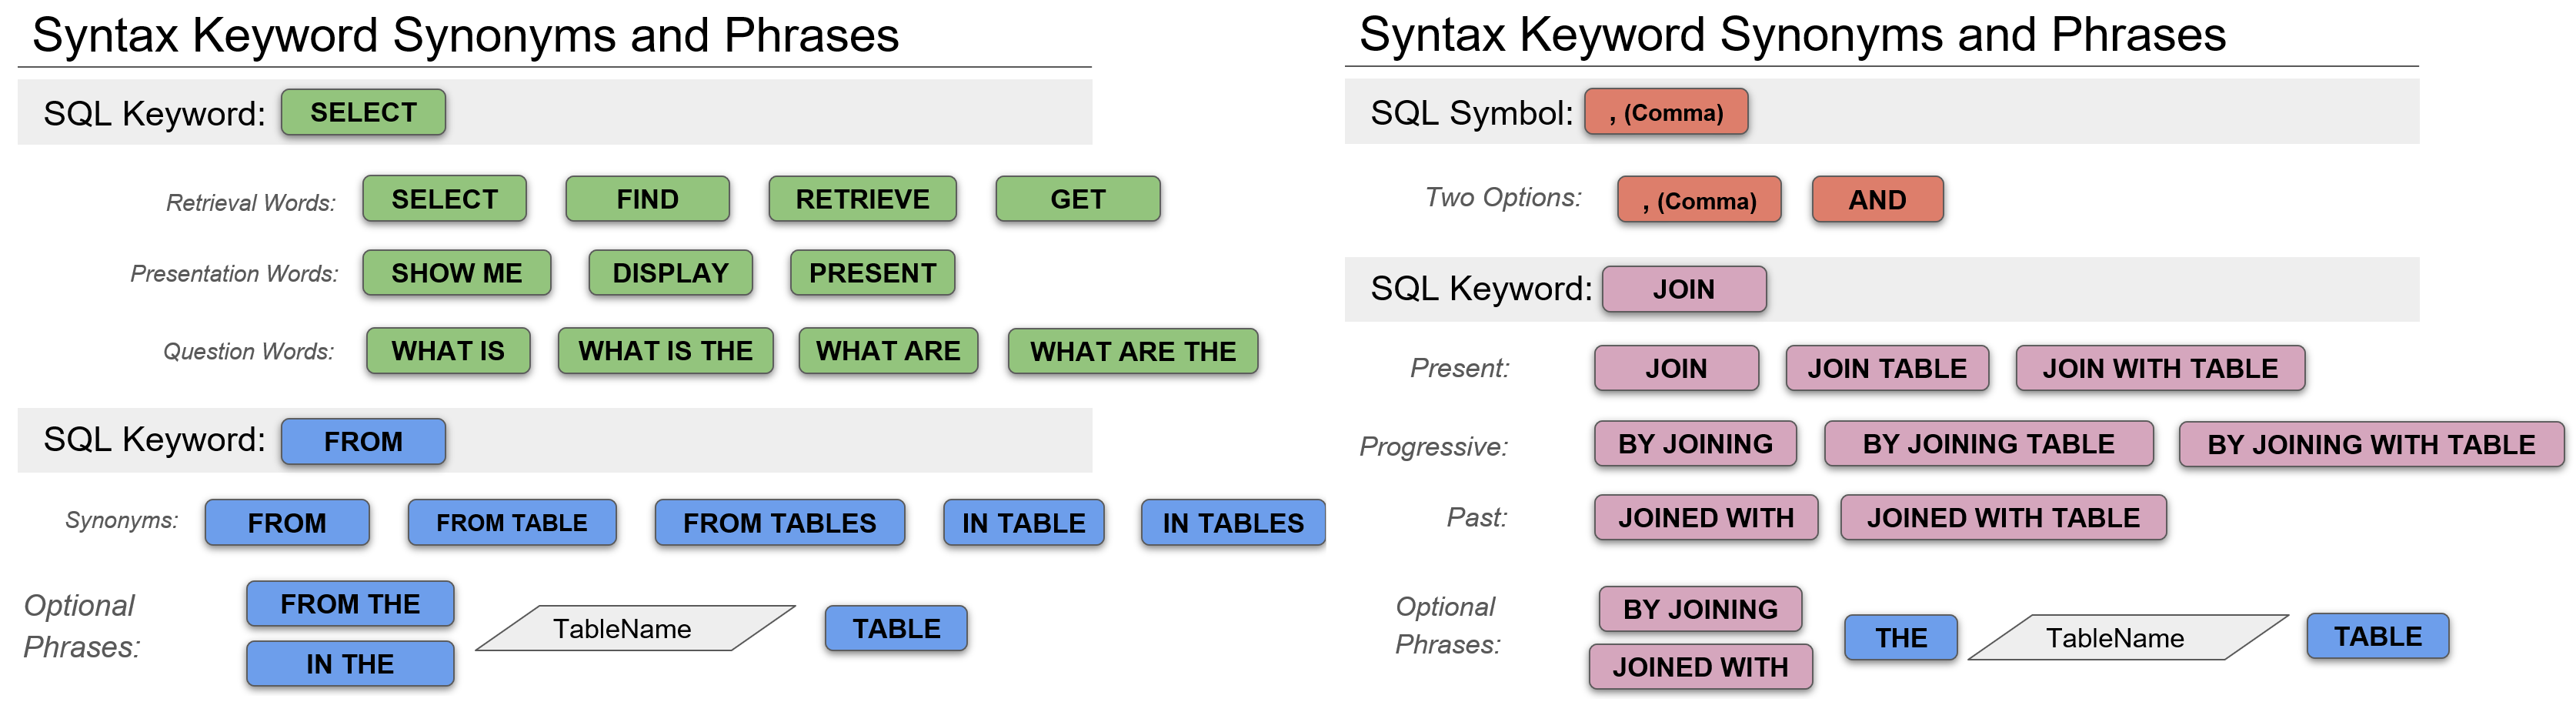
\includegraphics[width=\textwidth]{figures/all_synonyms.png}
  \caption{SpeakQL Synonyms}
\end{figure*}

Keyword synonyms are keywords with meaning equivalent to standard SQL keywords such as select, from, and join. The intent of this feature is to relax the rigidity of the formal SQL syntax and enable users to choose from several options when formulating queries. The standard SQL keywords remain within the vocabulary so users who are highly experienced with SQL may still use SQL syntax. The underlying idea that motivates this feature is that making equivalent keyword synonyms available using formal grammar rules offers more natural speech patterns, particularly in cases when other features such  as query reordering or unbundling of queries with multiple relations are used. For example, if a user elects to define the table relation prior to column projection, they may say "in table x" and follow  this statement with the keyword "find a, b and c" resulting in the statement "in table x find a, b and c." This statement is equivalent to the SQL query select a, b, c from table x. Table \ref{tab:keyword-synonyms} contains a list of SpeakQL keyword synonyms and their associated SQL keywords.

\subsubsection{Optional Syntax}

SpeakQL allows for the use of optional 'the' and 'table' keywords when dictating a table expression. This permits expressions such as 'select * from \emph{the} courseoffering \emph{table}', where the keywords \emph{the} and \emph{table} are optional additions that exist for the purpose of making table expression statements feel more natural for the speaker.

\subsubsection{Keyword Synonym and Optional Syntax Examples}

%Example query
\paragraph{SpeakQL} \emph{"\textbf{Show me} area and wheelchairspaces \textbf{in the} room \textbf{table} where floor = 2"}
\begin{verbatim}
  SQL: Select area, wheelchairspaces 
       from room where floor = 2;
\end{verbatim}

%Example query
\paragraph{SpeakQL:} \emph{"\textbf{What is the} count(id) \textbf{in the} course \textbf{table}"}
\begin{verbatim}
  SQL: Select count(id) from course;
\end{verbatim}

\begin{center}
  \begin{table}
  \begin{tabular}{|m{6em} m{18em}|}
    \hline
    \textbf{SQL Keyword} & \textbf{SpeakQL Synonyms} \\
    \hline
    SELECT & Select, Find, Retrieve, Get, Show Me, Display, Present, What Is, What Is The, What Are, What Are The \\
    \hline
    FROM & From, From table, From Tables, In Table, In Tables \\
    \hline
    ' , ' (Comma) & ' , ' (Comma), And \\
    \hline
    JOIN & Join, Join Table, Join With Table, By Joining, By Joining Table, By Joining With Table, Joined With, Joined With Table \\
    \hline
  \end{tabular}
  \caption{Keyword Synonyms}
  \label{tab:keyword-synonyms}
\end{table}
\end{center}

\subsection{Query Structure and Order Variance}

A standard SQL select expression must conform to the order \emph{Select -> From -> Join -> Where -> Group By -> Having -> Order By -> Limit}. SpeakQL's order variance permits additional orderings (see figure \ref{fig:alternate_ordering}) of expressions as well as the trailing select modifier clauses (see figure \ref{fig:selectmodifiergrammar}).

\begin{figure}[H]
  \centering
  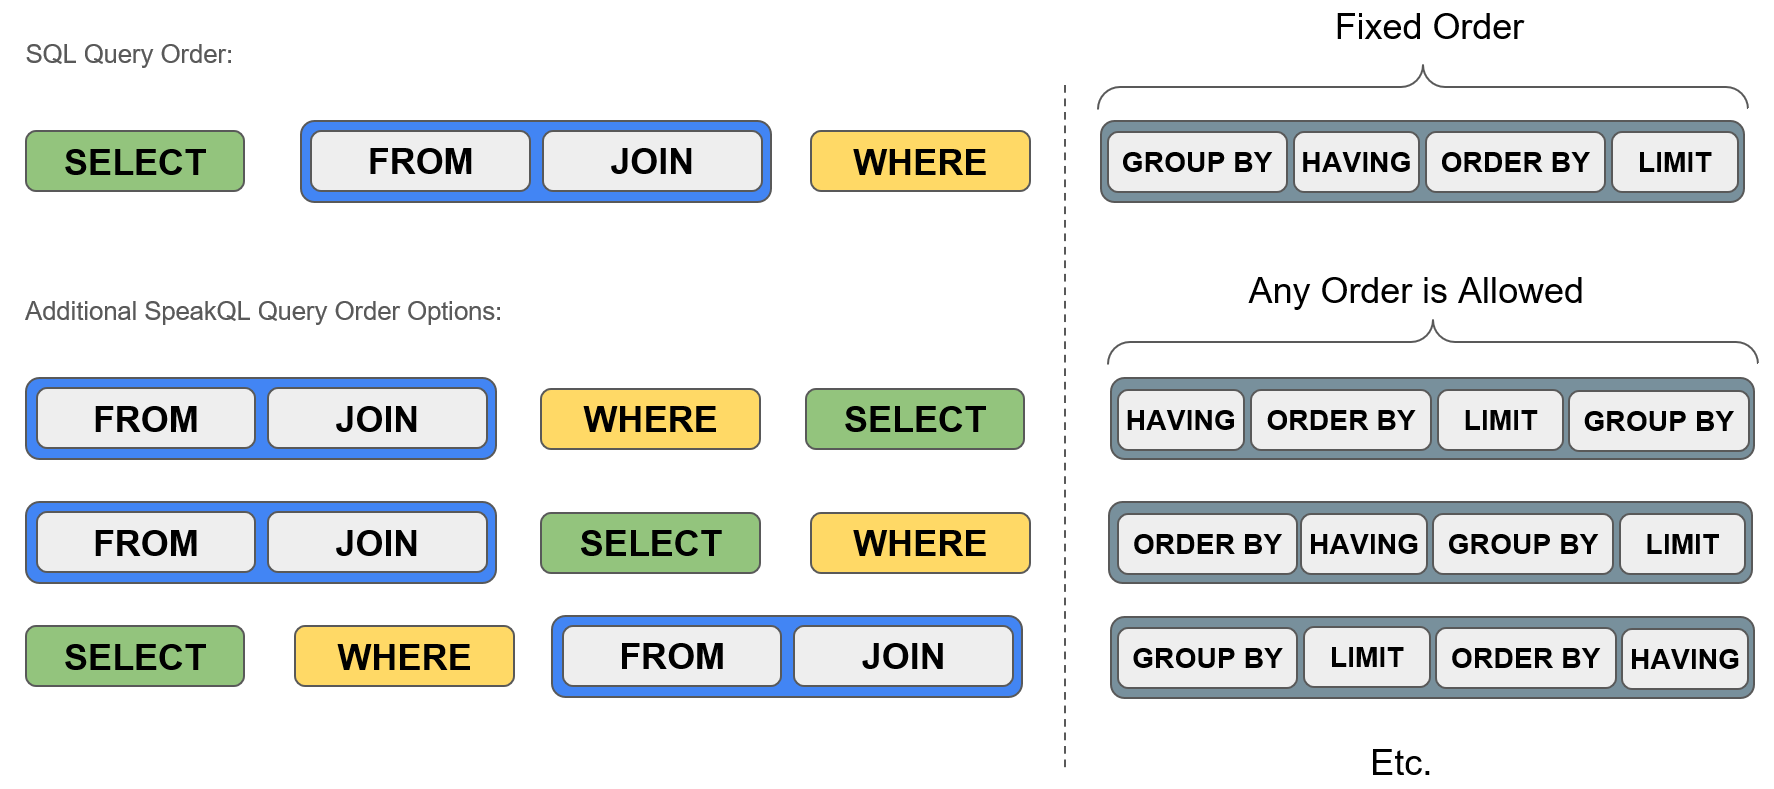
\includegraphics[width=\linewidth]{figures/alternate_ordering.png}
  \caption{Alternate Ordering}
  \label{fig:alternate_ordering}
\end{figure}

As with other features, the alternate ordering feature is optional. Query speakers may choose to conform to the standard SQL order specification. The alternate ordering provides options to query speakers who may be more comfortable with specifying source tables or where predicates prior to column selections or function specifications. We hypothesize that relaxing the order of the modifier clauses \emph{group by, having, order by, and limit} makes the query dictation process more error tolerant by transferring the responsibility for recalling the specific order of the clauses from the query speaker to the SpeakQL translator.S

\subsubsection{Alternate Ordering Examples}

%Example query
\paragraph{SpeakQL} \emph{"\textbf{From} term \textbf{show me distinct} termperiod  \textbf{table} where year = 2022"}
\begin{verbatim}
  SQL: Select distinct termperiod from term 
       where year = 2022;
\end{verbatim}

%Example query
\paragraph{SpeakQL:} \emph{"\textbf{In the} courseoffering \textbf{table where} capacity > 20 \textbf{find} facultyname \textbf{and} ondays \textbf{limit} 10 \textbf{order by} facultyname"}
\begin{verbatim}
  SQL: Select facultyname, ondays 
       from courseoffering 
       where capacity > 20 
       order by facultyname limit 10;
\end{verbatim}


\subsection{Natural Functions}

The SpeakQL 1.0 grammar includes aggregator functions such as \emph{sum, avg,} and \emph{count}, and query speakers are required to verbalize the parentheses symbols. While parentheses are essential for disambiguation in many traditional cases, for SpeakQL 2.0 we identified a set of function references where parentheses could be omitted without affecting the meaning of the query. Specifically, the SpeakQL dialect permits the expression of functions naturally, that is without verbalizing parenthesis, for functions that have only a constant or single column as an argument (See figure \ref{fig:naturalfunctions}). The natural function feature also permits optional syntax keywords \emph{the} and \emph{of} that surround the function name. 

In cases where a speaker's query intent requires the inclusion of an expression as a function argument, the verbalization of parenthesis remains a requirement. This allows the SpeakQL dialect to retain SQL's capability to pass mathematical, comparative, and subquery expressions as function arguments without these expressions introducing ambiguity.


\begin{figure*}
  \centering
  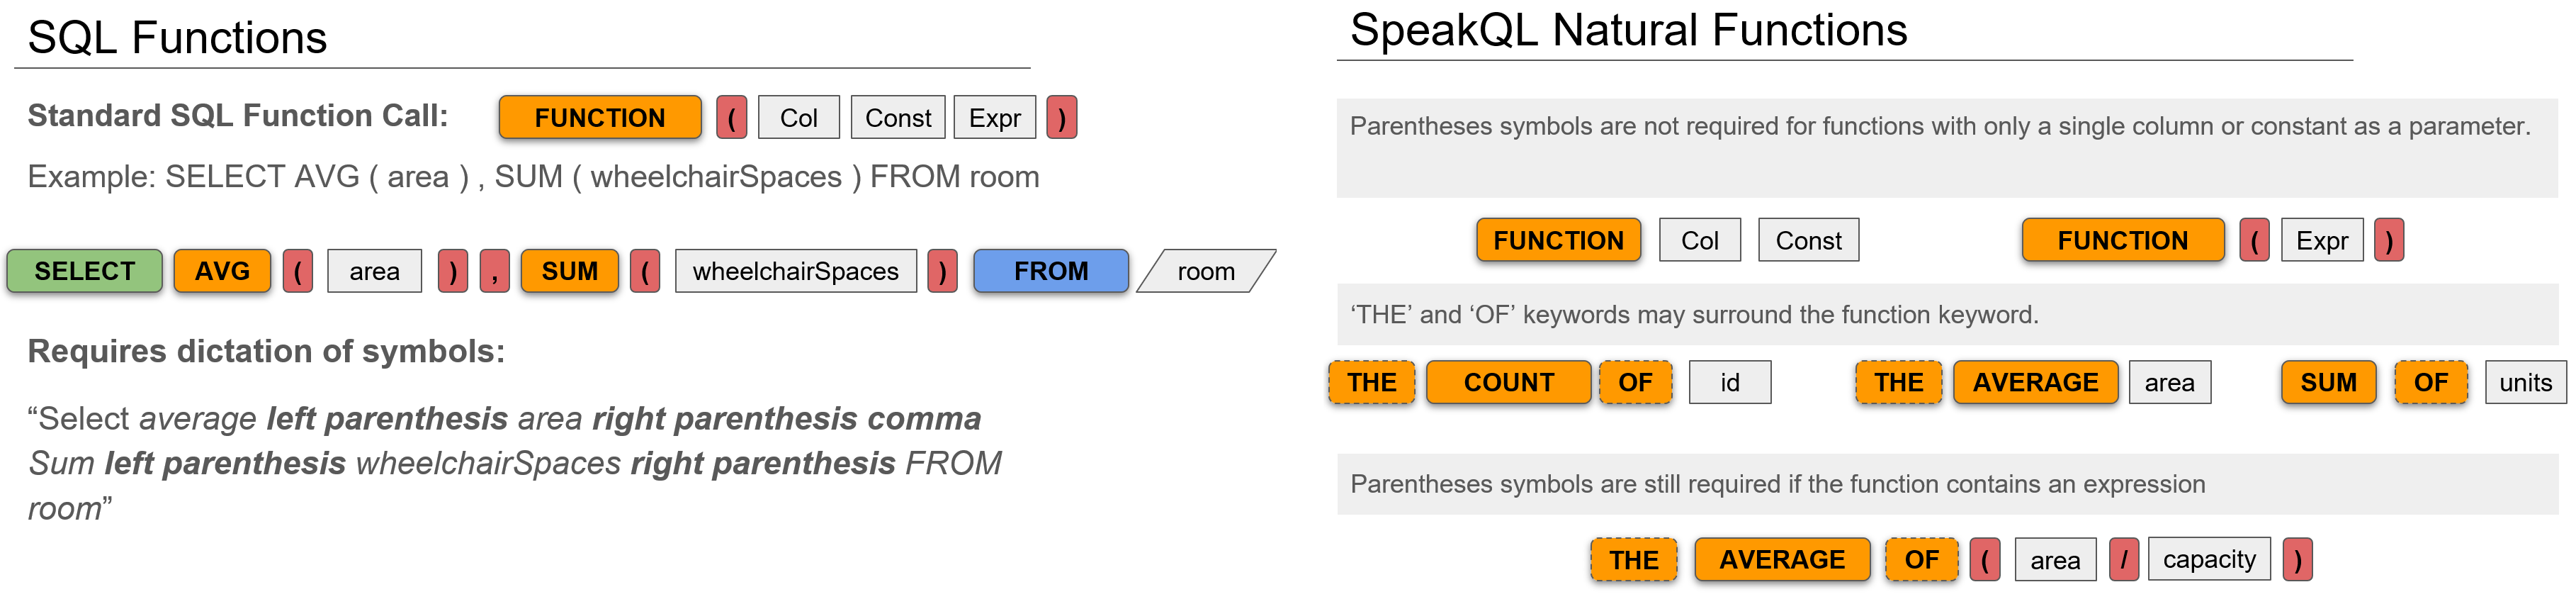
\includegraphics[width=\textwidth]{figures/natural_functions.png}
  \caption{Natural Functions}
  \label{fig:naturalfunctions}
\end{figure*}

\subsubsection{Natural Function Examples}

%Example query
\paragraph{SpeakQL} \emph{"\textbf{Get the count of} id \textbf{from the} course  \textbf{table}"}
\begin{verbatim}
  SQL: Select count(id) from course;
\end{verbatim}

%Example query
\paragraph{SpeakQL:} \emph{"\textbf{Find the average} units \textbf{and the count of} title \textbf{in the} course \textbf{table}"}
\begin{verbatim}
  SQL: Select avg(units), count(title)
       from course
\end{verbatim}

\subsection {Unbundling}

Query unbundling provides an alternative approach to complex query formulation. In standard SQL, the select expression requires query writers and speakers to specify all columns, scalars, and functions first before then proceeding to define table sources, subqueries, and joins, followed by expressing all restrictions in the form of where predicates. Only after this process has been completed may the query speaker then modify the expression with result row limits and ordering, apply selections to aggregate values using having, and grouping non-aggregate columns using the group by clause. This requires the retention of key information within a query speaker's working memory for the duration of the query dictation process. 

\begin{figure}[H]
  \centering
  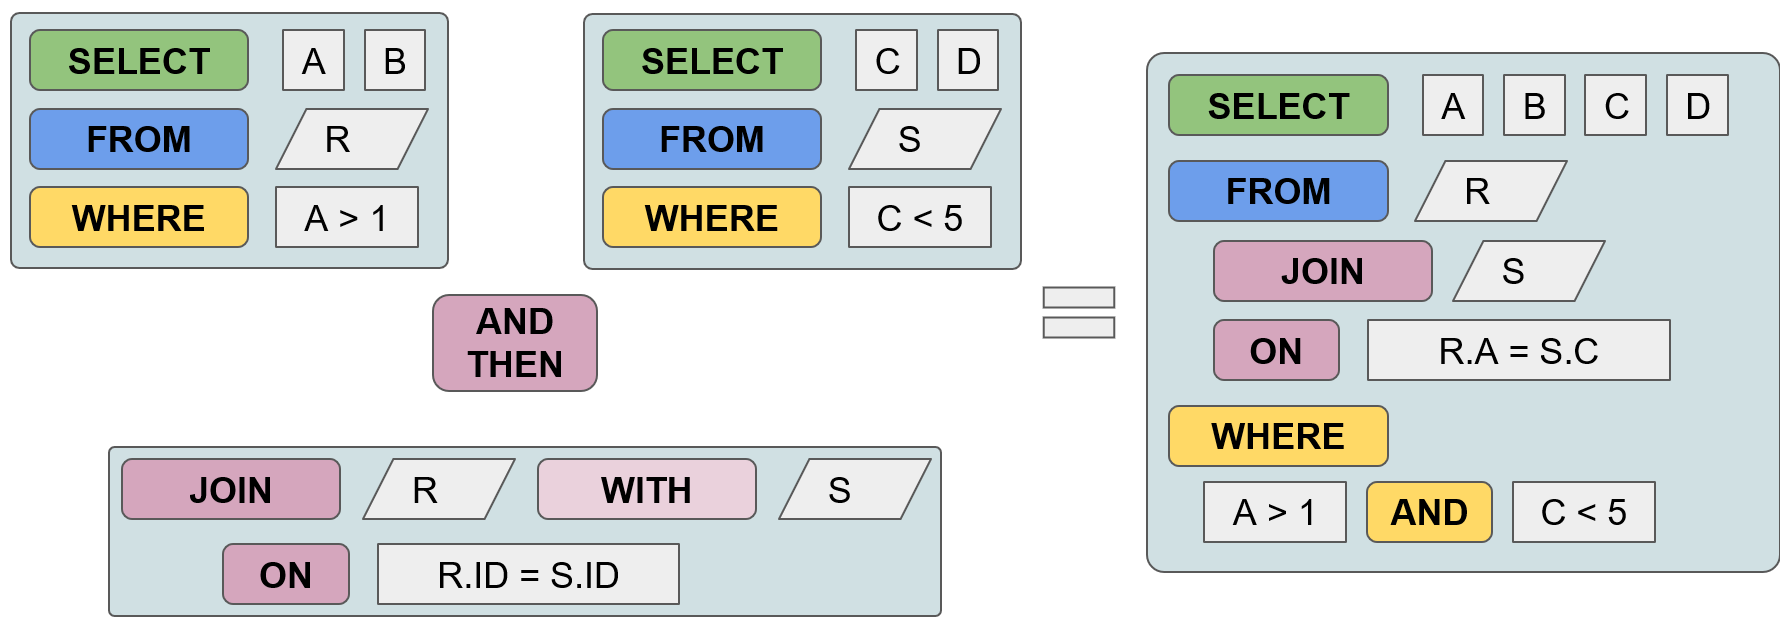
\includegraphics[width=\linewidth]{figures/unbundling_1.png}
  \caption{Query Unbundling}
  \label{fig:unbundling}
\end{figure}

The goal of unbundling is to reduce the cognitive load on query speakers by introducing a new grammar that permits the expression of \emph{unbundled select} subqueries that specify columns, table source, and where predicates for a single relation at a time. The tables specified in these unbundled queries are joined together using separate \emph{join-with} subqueries where query speakers define the relationship between two tables in their objective query. Modifier clauses may be specified together in a single expression, or seperately using multiple \emph{modifier} subquery expressions. The order of the \emph{unbundled select}, \emph{join-with}, and \emph{modifier} subqueries is optional, introducing additional flexibility to the query dictation process. Each unbundlined sub-query is delimited by the \emph{and then} keywords.

As the following examples will demonstrate, unbundled queries tend to contain more tokens than their corresponding SQL translations and are therefore longer and likely take more time to dictate. This is the result of decisions made within the trade space between the necessary brevity of keyboard-typed SQL and the natural flow of spoken language where SpeakQL introduces optional phrases and keywords to improve the dictation process. Therefore, we sacrifice some time-based efficiency in an effort to decrease the likelihood of semantic errors and improve the users' overall query dictation experience. 

\subsubsection{Unbundling Examples}

%Example query
\paragraph{Query Prompt} What is the average room seating capacity of rooms in buildings where the course with id 'CSE 232' has ever been offered? 

\paragraph{SpeakQL} 
\emph{
  "\textbf{Get} buildingname \textbf{from} building \\
  \textbf{and then}
  \textbf{from} room \textbf{where} floor = 3 \textbf{select average} capacity \\
  \textbf{and then}
  \textbf{select} nothing \textbf{from} courseoffering \textbf{where} courseid = 'CSE232' \\
  \textbf{and then}
  \textbf{join} courseoffering \textbf{with} room \textbf{on} courseoffering.roomid = room.id \\
  \textbf{and then}
  \textbf{join} room \textbf{with} building \textbf{on} room.buildingid = building.id \\
  \textbf{and then}
  \textbf{group by} automatically"
}


\begin{verbatim}
  SQL: Select buildingname, avg(capacity)
       from courseoffering
       join room on courseoffering.roomid = room.id
       join building on room.buildingid = building.id
       where courseoffering.courseid = 'CSE232'
       group by buildingname;
\end{verbatim}

%Example query
\paragraph{Query Prompt} Find the titles of all courses offered in terms with the year 2022. 

\paragraph{SpeakQL} 
\emph{
  "\textbf{join the} term \textbf{table with the} room \textbf{table on} term.id = courseoffering.termid \\
  \textbf{and then}
  \textbf{join the} courseoffering \textbf{table with the} course \textbf{table on} courseoffering.courseid = course.id \\
  \textbf{and then}
  \textbf{show me} title \textbf{in the} course \textbf{table} \\
  \textbf{and then}
  \textbf{from} room \textbf{where} floor = 3 \textbf{select average} capacity \\
  \textbf{and then}
  \textbf{get} nothing \textbf{from} term \textbf{where} year = 2022"
}
\begin{verbatim}
  SQL: Select title from course
       join courseoffering 
          on course.id = courseoffering.courseid
       join term 
          on courseoffering.termid = term.id
       where year = 2022;
\end{verbatim}


% \subsection{Multi-Feature Examples}
% \paragraph{Simple Queries}

% This is where we use the queries from the SpeakQL 1.0 paper \cite{Shah2020tr} to demonstrate new query ideas.
% \newline
% Natural Language Statement: Get starting dates of the employees who are working
% in department number d002.
% \newline
% Query 3: SELECT FromDate FROM DepartmentEmployee WHERE DepartmentNumber = 'D002'
% \newline
% Equivalent Natural Language Statement: From department d002 display employee 
% starting dates.
% \newline
% Equivalent SpeakQL 2 queries: 
% \begin{itemize}
%   \item In table DepartmentEmployee where DepartmentNumber = 'D002' find FromDate
%   \item From table DepartmentEmployee where DepartmentNumber = 'D002' Select FromDate
%   \item Show me FromDate in table DepartmentEmployee where DepartmentNumber = 'D002'
%   \item Retrieve FromDate from table DepartmentEmployee where DepartmentNumber = 'D002'
% \end{itemize}


% \paragraph{Complex Queries}




\section{SpeakQL 2 Implementation}


\begin{figure}
  \centering
  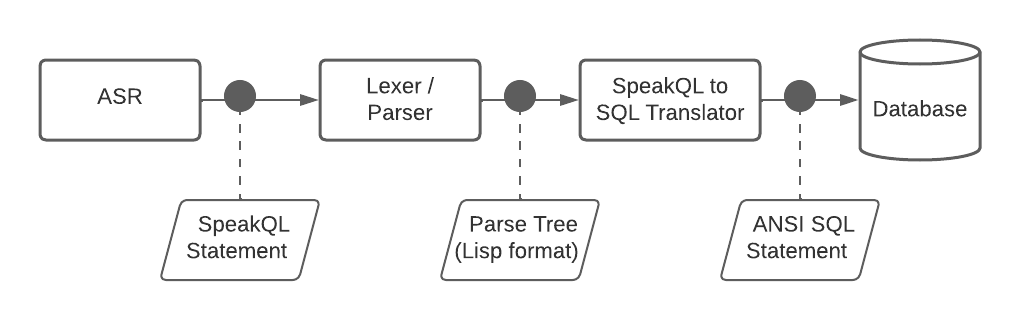
\includegraphics[width=\linewidth]{figures/SpeakQL 2 to SQL Translation}
  \caption{SpeakQL Dialect to ANSI SQL Translation Process}
\end{figure}

The objective of SpeakQL and SpeakQL 2 system implementations is to enable execution of SQL queries on arbitrary relational databases. We achieve this objective using the SpeakQL dialect by creating a SpeakQL dialect to SQL translator. This allows us to leverage existing database management systems and eliminates the requirement to create SpeakQL dialect-specific database engine optimisations. 


\subsection{SpeakQL Dialect Lexer and Parser}

We make use of ANTLR's implementation of ALL(*) \cite{Parr2014}, specifically the feature that enables context-based parsing using look ahead parsing to resolve potential ambiguity encountered while generating a statement's abstract syntax tree. That is, the parser recognizes its current location within the grammar and uses context to identify the parser rule associated with the next word in the query. This affords some flexibility in ordering of parser rules associated with SpeakQL features. For example, we add an intermediate rule layer between the SQL querySpecification rule and the SQL SELECT and FROM keywords, and title the associated rules in this layer selectExpression and tableExpression respectively. We can then create two alternate orderings (select then table, or table then select) both of which the parser recognizes as valid and correctly parses based on preceding and succeeding words in a given query.

\subsection{SpeakQL Dialect Grammar}

The SpeakQL 2 grammar is a modified extension of the MySQL grammar \cite{antlrgrammarsv4} described using the ANTLR language definition syntax. While the majority of the MySQL grammar remains unmodified, we make some significant adjustments within the \emph{selectStatement} and \emph{querySpecification} parser rules, which are rules within the dmlStatement rule set. Figures \ref{fig:queryexprgrammar}, \ref{fig:selectexprgrammar}, \ref{fig:tableexprgrammar}, \ref{fig:whereexprgrammar}, \ref{fig:selectmodifiergrammar}, \ref{fig:functiongrammar}, and \ref{fig:unbundlegrammar} portray most, but not all, of the grammar rules modified to enable SpeakQL dialect features. Most parser rule names appear in truncated form in the included figures, and some rules have been omitted based on their obscurity and lower likelihood of being used within a spoken query. The full grammar, including full parser rule names and rules not depicted in this paper, may be viewed in the ANTLR source files that define the full SpeakQL dialect grammar.

\subsubsection{Synonym and Syntactic Sugar Grammars}

To enable the synonym feature, we create additional keyword parser rules as intermediate rules within the SpeakQL parser that contain multiple keyword synonyms. For example, the selectKeyword parser rule contains the select synonym keywords (e.g. \emph(get, display, show me) etc.). Parser rules \emph{selKW}, \emph{joinKW}, and \emph{frmKW} in Figures \ref{fig:selectexprgrammar}, and \ref{fig:tableexprgrammar} exist one level above terminal representative of each SpeakQL synonym. These keyword-based intermediate parser rules provide the SpeakQL-to-SQL translator with a reference point for keyword replacement as depicted in algorithm \ref{alg:synonyms}.

\subsubsection{Alternate Ordering Grammars}
Parser rule queryOrdSpec (query order specification) in Figure \ref{fig:selectexprgrammar} contains four branches representing the four alternate ordering options for the select statement's \emph{select}, \emph{from-join}, and \emph{where} expressions. The selModExpr (select modifier expression) also in Figure \ref{fig:selectexprgrammar} contains a single branch that contains four optional rules that serve as placeholders for any of the four modifier clauses \emph{group by}, \emph{having}, \emph{order by}, and \emph{limit}. This approach differs from the select expression branching due to the increased number of ordering options. Because each placeholder rule can contain any of the modifier clauses, the SpeakQL-to-SQL translater assumes the responsibility for addressing cases where a query speaker incorrectly specifies more than one limit clause or conflicting order-by clauses.

\subsubsection{Natural Function Grammars}

The SpeakQL grammar retains the \emph{functionCall} parser rule in the original MySQL grammar from which it was derived, and adds an additional child rule as a sibling to the \emph{aggregateWindowedFunction} parser rule that specifies functions commonly used to fulfill analysis-focused tasks (e.g. \emph{count}, \emph{sum}, etc.). The additional sibling rule, titled \emph{noParenAggregateWindowedFunction}, contains a subset of the functions available in the \emph{aggregateWindowedFunction} parser rule. Additionally, as depicted in figure \ref{fig:functiongrammar}, the \emph{functionArg} parser rule which enables a wide range of rules to exist as parameters, is replaced by a more restrictive rule that allows only \emph{constant} and \emph{columnName} rules to exist as legal children rules that follow the name of the function. This constraint mitigates unintended ambiguity may occur when attempting to specify a complex expression without surrounding parentheses. 

\subsubsection{Unbundling Grammars}

Our approach to defining unbundling grammar involves the creation of additional rules (see figure \ref{fig:unbundlegrammar}) that delimit between unbundled expressions (\emph{expressionDelimiter}), restrict the use of joins within the from clause (\emph{fromClauseNoJoin}), and define a standalone join expression (\emph{multiJoinExpression}) that employs the \emph{withKeyword} rule to specify a join relationship between two tables or subqueries. Unbundled grammar is accessed at a relatively high level in the SpeakQL grammar from the (\emph{querySpecification} parser rule (see figure \ref{fig:queryexprgrammar}). 

Generally, the parser will recognize that a specific query is employing unbundling features when the query speaker specifies an \emph{expressionDelimiter} token (e.g. \emph{and then, then, or next}) between two unbundled subqueries. Once this occurs, the parser will only recognize queries as legal if they do not contain join expressions within the table expression, as all joins in unbundled queries must be defined using the \emph{multiJoinExpression} parser rules. Although not expected to occur often, unbundled queries may contain subqueries in lieu of table names. These subqueries do not necessarily have to conform to the unbundled syntax, and may follow either the unbundled or non-unbundled paths through the grammar.

\begin{figure}
  \selectStatementTable
  \caption{Query Expression Grammar}
  \label{fig:queryexprgrammar}
\end{figure}

\begin{figure}
  \selectExpressionTable
  \caption{Select Expression Grammar}
  \label{fig:selectexprgrammar}
\end{figure}

\begin{figure}
  \tableExpressionTable
  \caption{Table Expression Grammar}
  \label{fig:tableexprgrammar}
\end{figure}

\begin{figure}
  \whereExpressionTable
  \caption{Where Expression Grammar}
  \label{fig:whereexprgrammar}
\end{figure}

\begin{figure}
  \selectModifierTable
  \caption{Select Modifiers Expression Grammar}
  \label{fig:selectmodifiergrammar}
\end{figure}  

\begin{figure}
  \naturalFunctionTable
  \caption{Function Call Grammar}
  \label{fig:functiongrammar}
\end{figure}  

\begin{figure}
  \unbundleQueryTable
  \caption{Unbundling-Related Grammar Rules}
  \label{fig:unbundlegrammar}
\end{figure}  

\begin{figure}
  \sqlSelectStatementTable
  \caption{SQL Select Statement Grammar Excerpt}
  \label{fig:sqlselectgrammar}
\end{figure}

\subsection{SpeakQL Query to SQL Query Translation}

The SpeakQL to SQL translation process begins with a parse operation on a valid query expressed in the SpeakQL dialect. For purposes of translation, we assume that an automatic speech recognition (ASR) and error correcting application has resolved any query dictation or speech recognition errors that may have occurred. In other words, the SpeakQL translator assumes that the tokens present in the query reflect the intent of the query writer. 

The result of the query parsing operation is an abstract syntax tree (AST) containing the grammar rules associated with the statements present within the query. The AST is initially generated using a Java-based SpeakQL parser specified using the ANTLR \cite{Parr2014} language. The Java-based result is passed to the Python-based translator as a Lisp-style tree. On receipt of the lisp tree, the translation begins when the translator parses the lisp tree and generates a Python-based AST.

Upon initialization, the Python-based AST performs cataloguing operations including cataloging and masking subqueries, generating a dictionary of referenced tables and aliases, generating a list of referenced columns, and generating a two way table-column dictionary. Tree nodes are indexed in a dictionary-based data structure, and nodes-to-node associations exist in the translator as index references enforced by the tree node index. During initialization, the translator also generates statistics useful for determining if specific translation features need to be executed on a given query.

After AST initialization is complete, the translator begins the translation process. The result of this process is a re-ordered AST that, when serialized, outputs a valid SQL query. This is accomplished through a series of steps: replacing SpeakQL synonyms with equivalent SQL keywords, re-ordering expressions into valid SQL expression order, removing syntactic sugar, and bundling unbundled queries. These operations are performed recursively on any subqueries cataloged during initialization.

\subsubsection{Synonym Replacement}

Synonym replacement, where SpeakQL keywords are replaced with equivalent SQL keywords, occurs as the first step of query translation. To accomplish this task, the translator performs a scan search of all active nodes in the AST for rules that are a member of the keyword and delimiter categories for which SpeakQL synonyms exist. This includes \emph{selectKeyword}, \emph{fromKeyword}, \emph{selectElementDelimiter}, and others. When a keyword or delimiter rule is identified during the search, the translator performs an update on the rule node which replaces the terminal token representative of a SpeakQL synonym with its corresponding SQL keyword.

\begin{verbatim}
  SpeakQL rule:      'selectKeyword SHOW ME'
  After replaceKW:   'selectKeyword SELECT'
\end{verbatim}

Algorithm \ref{alg:synonyms} provides a pseudo-code representation of the synonym replacement process performed by the translator on the SpeakQL AST. After completion, all SpeakQL synonym keywords that existed in the initial query and its subqueries have been replaced with valid SQL syntax.

\ReplaceSynonymsAlgorithm

\subsubsection{Expression Reordering}

The next step of the translation process is expression reordering. This step includes both the reordering of \emph{select, from, where} and \emph{group by, order by, having, limit} expressions. For this feature, we take advantage of the grammar structure and associated AST structures that guarantees that all children of the \emph{queryOrderSpecification}, \emph{unbundledQueryOrderSpecification}, and \emph{selectModifierExpression}, parser rule nodes are rules that should be evaluated and reordered. Specifically, we can be certain that the query order expression parser rules will only contain the children \emph{selectExpression}, \emph{whereExpression}, \emph{tableExpression}. We are also certain that the \emph{selectModifierExpression} has no more than four children of type \emph{selectModifierItem}, each of which may have only one child of type \emph{groupByClause}, \emph{havingClause}, \emph{orderByClause}, or \emph{limitClause}. These guarantees enable us to limit the scope of reordering operations to only the children of the parent nodes of the sub-expressions. 

Algorithm \ref{alg:reorder} portrays the process by which the translator modifies the AST. Expression reordering is accomplished by iteration over the array containing the children of \emph{queryOrderSpecification}. When the first rule in the SQL order (\emph{selectExpression}) is encountered, this node is added to a new children list object. Iteration over the remaining children rules continues until all children have been identified and reordered into the new children list in SQL-correct order. The translator then updates the parser rule node \emph{queryOrderSpecification}, replacing its old children list with a new list containing the same children, but in SQL-correct order.

\ReorderParseTreeAlgorithm

Algorithm \ref{alg:reordermodifiers} portrays a similar process that reorders what we refer to the select modifier rules which includes \emph{groupByClause}, \emph{havingClause}, \emph{orderByClause}, and \emph{limitClause} parser rules. The translator employs the same strategy of iteration over the parent rule's children, except that it must descend one level deeper through the additional intermediate layer consisting of up to four \emph{selectModifierItem} rules that exist between the parent \emph{selectModifierExpression} and child clause parser rules. The translator iterates over the original child list and places the clauses in SQL-correct order into a new list. After iteration is complete, the \emph{selectModifierExpression} children are replaced with the SQL-ordered list of select modifier clauses.

\ReorderModifiersAlgorithm

\subsubsection{Natural Function Transformation}

The SpeakQL natural functions feature allows for the omission of parentheses and the inclusion of optional \emph{the} and \emph{of} keywords for functions where only a single column or constant value is passed as argument. Translating natural functions to SQL-correct function statements involves the removal of the optional keyword parser rules and the insertion of parentheses. The translator's AST class contains helper functions \emph{removeNodeFromTree} and \emph{surroundNodeWithParens} used to accomplish these tasks.


\subsubsection{Query Bundling}

Query bundling is the series of tasks the translator performs to combine a set of unbundled queries into a valid SQL statement. 
  
\TransformUnbundledQuery

At a high level, this is accomplished through a series of up to five steps (see algorithm \ref{alg:transformunbundled}). The actual number of steps executed for a given query depends upon the existence of certain statements within the query. For example, the \emph{inferGroupBy} step will be skipped for queries that do not contain aggregator functions and an associated group by expression. However, every valid SpeakQL query that employs unbundling will, at a minimum, execute the \emph{bundleSelectElements}, and either \emph{bundleJoinParts} or \emph{bundleTables} methods. Unbundling steps are performed in the order:

\begin{enumerate}
  \item Infer group by expression (optional)
  \item Bundle select elements
  \item Bundle where statements (optional)
  \item Bundle join parts (optional)
  \item Bundle tables (optional)
\end{enumerate}

The translator generally uses the same approach for each bundling step, which is to identify the first expression parser rule node in the AST for a given expression and use it as a migration target for additional expression parser rule nodes that may exist in the AST. For example, if a query contains two separate unbundled select-from-where queries connected with a join query, the translator will designate the first of the two \emph{selectExpression} parser rules in the AST as \emph{selectExpression'} and will migrate the \emph{selectElements} that are children of the second \emph{selectExpression} rule node to become children of \emph{selectExpression'}. Additional considerations apply individually to each bundling step, and will be discussed in more detail in the step-specific paragraphs that follow. Parser rule node migration is accomplished by appending the migrated parser rule node's ID to the migration target rule node's child list and removing the migrated parser rule node's ID from the migration source rule node's child list.

\paragraph{Inferring the group by expression}

A feature of the SpeakQL translator is its ability to infer a group by expression using the presence of aggregator functions and column references within multiple \emph{selectExpression} parser rules. A user can instruct the translator to perform group by expression inference using the \emph{group by automatically} keyword within either a single-table SpeakQL query or a multi-table unbundled query.

\TransformFunctionInferGroupBy

When the translator encounters the \emph{group by automatically} instruction, it proceeds as depicted in algorithm \ref{alg:infergroupby}. It makes use of AST helper functions \emph{nodeWithName} which returns a list of all nodes with a given rule name, and \emph{getAllTablesAndElements} which returns a Python dictionary (\{ \emph{table name} : [ \emph{selectElements} ]\}) that contains a list of select elements and function calls for each table referenced within the SpeakQL query. The translator uses the existing \emph{groupByExpression} parser rule node that contains the \emph{auomaticGroupByKeyword} parser rule and replaces the \emph{automaticGroupbyKeyword} rule with a \emph{groupByItems} parse rule. The \emph{groupByItems} parse rule node serves as the parent node for individual \emph{groupByItem} and \emph{groupByItemDelimiter} nodes generated from non-function \emph{selectElement} nodes registered in the table-element python dictionary. Because the \emph{groupByItems} parse rule already exists beneath the \emph{selectModifierExpression} parse rule, no further AST transformations are required; and the group by inference operation is complete after the generation of the \emph{groupByItems} parse rule and its children \emph{groupByItem} and \emph{groupByItemDelimiter} parse rules.

\paragraph{Bundling select elements}

Select element bundling is a required step for any SpeakQL query that makes use of the unbundling feature. Because any SpeakQL query that uses unbundling must have at least two \emph{selectExpression} parse rules, select element bundling is a mandatory step of the bundling process.

\TransformFunctionSelectElements

As shown in algorithm \ref{alg:transformfunctionselectelements} as \emph{selElmtsRlNd'}, which abbreviates \emph{selectElementsRuleNode}, the translator uses the first \emph{selectElements} parser rule as a migration target for all other select elements within the SpeakQL query. Also depicted in the same algorithm is a preemptive method for avoiding ambiguity where the translator prepends each migrated select element with its associated table, resulting in a dotted id in the format \emph{tableName.columnName}. This step is performed for both standalone column references and column references as arguments within function expressions. After iterating through each \emph{selectElementExpression} parser rule and migrating their associated \emph{selectElements} children to \emph{selectElementsRuleNode'}, a cleanup operation removes them from the AST leaving a single \emph{selectElementsExpression} in the AST that contains all column and function references present in the original SpeakQL unbundled query.

\paragraph{Bundling where expressions}

The where expression bundling step is optional, and is only invoked if at least one bundled query expression contains a \emph{whereExpression} parse rule. When performing where expression bundling, the SpeakQL translator makes the following assumptions:

\begin{itemize}
  \item All cross-table predicates are conjunctive (and)
  \item Multiple predicate expressions within a single unbundled query should be encased in parentheses before consolidation
\end{itemize}

Given these assumptions, where expression bundling proceeds as depicted in algorithm \ref{alg:transformfunctionwherestatements}.

\TransformFunctionWhereStatements

Similar to the select element bundling step, the first occurence of a \emph{whereExpression} parse rule, \emph{whereExpression'}, within the query AST and designates it as the target for additional \emph{whereExpression} parse rule migration. Because where expressions are optional within \emph{selectStatement} parser rules, it is possible that \emph{whereExpression'} is not a member of the first \emph{selectStatement} parse rule, \emph{selectStatement'}, in the query. Because of this possibility, the translator may perform an additional migration step where it migrates \emph{whereExpression'} to become a child of \emph{selectStatement'}.

The translator takes advantage of the recursive nature of the where expression grammar (see figure \ref{fig:whereexprgrammar}) by designating where expressions that exist in \emph{selectStatement} parse rules that are not \emph{selectStatement'} as children of \emph{whereExpression'}. During this migration process, the translator employs helper functions to surround migrated expressions with parentheses and deliminating the migrated expressions with \emph{andKeyword} parser rules. The end result of this process is a single cross-table conjunctive \emph{whereExpression} parser rule that contains all other \emph{whereExpression} parser rules specified in other unbundled queries within the SpeakQL query. 

\paragraph{Bundling join parts}

Join part bundling collects all \emph{multiJoinExpression} parse rules and aggregates them in an arbitrary order to form a valid SQL join expression. Join part bundling is an optional feature because an alternate form of relation joining where all table sources are specified within \emph{fromExpression} parse rules, and join conditions between each table source are specified within \emph{whereExpression} predicates (e.g. \emph{from table one, table two where one.id = two.id}), is also possible. Currently, because join order in the resulting SQL query is arbitrary within the bounds of its implementation rules, join part bundling is limited to allowing only inner joins. Queries that require outer join expressions may still be expressed using other SpeakQL features; but may not employ the unbundling feature. Outer join capability is a future SpeakQL feature development objective.

% \TransformFunctionJoinParts

The join part bundling process begins when the translator creates a list of all \emph{multiJoinExpession} parse rule nodes within the AST. Given this list, it performs iterative analysis on each expression to determine if a subquery exists as a table item within any of the \emph{multiJoinExpression} nodes, and if so, substitutes the subquery with a subquery masking rule and alias in the join expression. The translator then checks the left and right table reference parse rules within the join expression to determine if an alias exists for each table, or if the table is referenced in the join expression by its alias. If an alias association is encountered, it creates \emph{asKeyword} and \emph{multiJoinTableAlias} parse rules and adds them as children to the target \emph{joinExpression} parser rule that represents the objective SQL-correct join expression.

After analyzing all \emph{multiJoinExpression} and making modifications toward SQL-correct syntax, the translator begins the join consolidation process by designating the first table referenced in the queries first \emph{selectStatement'} as the base table upon which the SQL-correct join statement will be built. In order to ensure valid join expression chaining, the translator determines a table join order that ensures that each subsequent table added to a join expression references a table in its join condition that already exists within the objective join expression. In other words, while building the SQL-correct join expression, a \emph{multiJoinExpression} will not be added to the target \emph{joinExpression} until all tables referenced in its join condition have been added to the target \emph{joinExpression}. The process will continue iterating over remaining \emph{multiJoinExpressions} until the table existence constraint can be satisfied and all expressions have been added to the objective SQL-correct expression, or it is determined that \emph{multiJoinExpressions} exist in the SpeakQL query that cannot be chained and the translator responds with an error condition. The translator then performs an additional safety check to ensure that all tables referenced in the query's \emph{unbundledQueryOrderSpecification} parser rules are also referenced in a corresponding \emph{multiJoinExpression} parser rule, and throws an error if a violation is encountered.

After the join bundling process is completed, all join expressions consolidated within a single \emph{multiJoinExpression} are migrated to the first \emph{tableExpressionNoJoin} parse rule. The \emph{tableExpressionNoJoin} parse rule name is then updated to \emph{tableExpression} and becomes a valid SQL from + join expression; and join bundling is complete.

\paragraph{Bundling table expressions}

The final step of the bundling process involves collection of all \emph{tableExpressionNoJoin} parse rule nodes within the AST. This is only required in cases where an unbundled query contains multiple table references but has no associated \emph{multiJoinExpression} parser rules. In this case the first \emph{tableExpressionNoJoin}, designated as \emph{tableExpressionNoJoin'}, is established as the expression migration target, and additional \emph{tableExpressionNoJoin} rules that exist as children of additional \emph{selectStatement} rules are added to \emph{tableExpressionNoJoin'}. If a where expression exists in any \emph(selectStatement) that defines a join condition between two tables within the query, the expression consolidation occurs during the previously described where expression bundling step. If no where condition is defined between two tables within the query, the translator still performs table expression bundling, and the result is a SQL statement that produces a cartesian product of the two tables.

% \TransformFunctionTables

\paragraph{Syntax tree cleanup}

After all relevant bundling steps are complete, the translator performs syntax tree cleanup by removing parse rules from which their child sub expressions have been migrated. Upon completion of tree cleanup, the SpeakQL to SQL translation process is complete, and serialization of the abstract syntax tree's terminal nodes results in a valid SQL statement equivalent to the input SpeakQL query.


\section{SpeakQL 2 Dialect Evaluation}


We are currently implementing a mixed-methods, within-subjects, comparative usability study of the SpeakQL 2 prototype language features by recruiting participants with SQL experience to spend approximately 90 minutes watching an instructional video and answering 12 questions using both SQL and SpeakQL 2. Our objective was to identify which, if any, SpeakQL 2 dialect features made the process of dictating queries easier and / or reduced the likelihood of errors.

\subsection{Objectives}

\subsubsection{Research Questions}

Our questions related to the structure and content of the proposed SpeakQL 2 dialect. Given the preliminary features for the SpeakQL dialect, and we sought to determine which of them actually improved the query dictation process.

\paragraph{Q1 - Effectiveness of alternate syntax:} To what extent, if any, does introducing syntax synonyms improve the user experience of constructing a query using speech recognition software?

\paragraph{Q2 - Effectiveness of alternate structure:} To what extent, if any, does altering the structure and order of SQL statements reduce the tendency for errors when constructing a query using speech recognition software?

\paragraph{Q3 - Effectiveness of unbundling:} To what extent, if any, does unbundling a complex query into smaller relation-focused parts reduce the possibility of failing to produce a valid query using speech recognition software?

\subsubsection{Hypotheses}

\paragraph{H1 - Synonyms and Reduction in Special Characters Improve User Experience} Introducing syntax synonyms and removing the requirement to speak special characters like 'comma', 'parenthesis', or 'asterisk', makes speaking a query feel more natural and improves user experience and reduces the number of errors and time taken to form simple queries.

\paragraph{H2 - Alternate Ordering Reduces Errors} Relaxing the ordering requirement for various subexpressions reduces the likelihood of ordering-based syntax errors and thus reduces the amount of time and number of attempts required to dictate a correct simple or complex query. 

\paragraph{H3 - Unbundling Unburdens Working Memory} As the number of tables and corresponding column references in a query increases, so does the probability of error when speaking a query. Breaking a complex, multi-table query into a series of individual single-table queries reduces the query speaker's working memory burden and reduces the likelihood of errors when constructing a query using speech recognition software. This should reduce the number of attempts required to form a correct complex query containing multiple relations.

\subsection{Protocol}

\subsubsection{Participants}

We have currently conducted 17 study sessions, 11 of which were with participants who were graduate students in data or computer science, one undergraduate computer science student, two senior professionals, and one junior professional. Two participants opted not to disclose any demographic or career information. We primarily targeted university programs that focus on analytics, and computer and data science. Because the SpeakQL dialect is an extension of the SQL syntax, we sought out participants who were already experienced with SQL which reduced the time required for training. Prospective participants were asked to complete a short SQL skills assessment, those who passed the screening questionnaire were then invited to participate in the experiment.

\subsubsection{Study Design}

\paragraph{Context} 

As both a COVID safety measure, and in an effort to recruit from as broad a pool as possible, the entire study is being performed online using a video conferencing program and a custom-built browser-based user interface. The  user interface enables participants to view a database schema, receive query prompts, dictate their queries through their device's microphone, and review a speech-to-text transcription of their dictation. The research facilitator uses a seperate 'wizard of oz' study control panel to evaluate user performance in terms of query correctness, provide feedback, answer SQL- and SpeakQL-related questions, and manage the progression of the study. 

\paragraph{Quantitative Analysis}

We evaluate performance using:

\begin{itemize}
  \item Total-Time-to-Completion: Lower is better. Total time (in seconds) from when the participant is presented with the question prompt to when they press the submit button for their final query submission.
  \item First Attempt Planning Time: Lower is better. Time (in seconds) from when the participant is presented with the question for the first time to when they press the record button.
  \item Dictation (recording) Time: Lower is better. Time (in seconds) from when the participant presses the record button to when they press the stop button.
  \item Number of Attempts: Lower is better. Discrete (1, 2, 3) inicating how many attempts the participant made to form a correct query.
\end{itemize}

We measure these variables both in terms of overall averages (mean) within each set, as well as percent change between dialects for each SpeakQL-SQL response pair used to answer a question. The latter approach mitigated the increased variance caused by the intermixing of simple and complex queries within the question set.

\begin{itemize}
  \item Query Complexity: Continuous positive real number derived from the presence and quantity of columns, tables, joins, functions and predicates. 
  \item Query is Complex: Discrete (0, 1) simpler method for indicating if a query is complex. Based on complexity threshold defined below.
  \item Query Attributes: Number of projections, number of tables, number of selections, number of joins, and number of modifiers required to answer the question.
  \item Features Used: One-hot encoded vector representing the SpeakQL features actually used by a participant for a given SpeakQL query.
\end{itemize}

\paragraph{Determining Feature Usage} We analyze feature usage in each query attempt by performing speech-to-text transcription on attempt recordings. The speech-to-text service was provided by an Amazon Web Services Transcribe custom language model trained on 500,000 procedurally generated SpeakQL and SQL queries against the same database used in the study.

\paragraph{Measuring Query Complexity} Query complexity is determined using a series of weighted criteria that include the number of tables (relations) in a query, the number of projections (columns, functions and constants within the select expression), number of functions, number of selections (where expressions), number of joins, and number of modifiers (group by, having, order by and limit). A query is considered to be complex if the standardized sum of the weighted criteria for a query is greater than 0. 

\[Complexity = Standardize(\sum_{i = 1}^{n} Weight_{i}*Score_{i})\]

Where \(Weight\) is a vector length \(n\) of weights associated with values in vector \(Score\) of length \(n\) and the standardization function computes a value between -1 and 1 using the complexity score of a query minus the mean divided by the standard deviation of all query complexity scores.

\[Standardize(WeightedScore) = \frac{WeightedScore - \mu_{Scores}}{\sigma_{Scores}}\]

\paragraph{Data Collection}

Data generated by the study includes time to plan (time from updating the query prompt until pressing record), time to record (time from pressing record to stopping the recording), number of attempts per query, dictation transcript, and audio recordings of each dication attempt. All data is captured within participants' browser sessions and uploaded to a back end web server and database for processing and analysis during the session. In an effort to add explanatory power to our quantitative results, we ask participants to complete a voluntary post-participation survey. 

\paragraph{Managing the Learning Effect}

We applied a latin squares approach using counterbalancing to counteract the learning effect \cite{10.5555/2501707} inherent in within-subjects studies of two or more treatments. Specifically, participants were divided into two groups: a SpeakQL-to-SQL group and a SQL-to-SpeakQL group, where participants in one group answered all 12 questions in one dialect and then switched to the opposite dialect and answered the same 12 questions again. Post-participation analysis confirmed the efficacy of this control by verifying that little-to-no assymetric learning occurred between dialects.

\subsection{Current Results}

So far we have collected 213 observations (query dictations) from 17 participants over the span of 120 days. 15 of the 17 participants opted to complete our post-participation survey.

\paragraph{Recording time} Running a generalized linear model using recording time as dependent variable and query attributes (number of functions, number of tables, number of projections) as independent variables revealed that speakql recording time increased by .06 (6 percent) for every table in the function (p = 0.005), and decreased by .17 (17 percent) (p = 0.001) for every function in the query.

\paragraph{Number of Attempts} On average, SpeakQL queries required .43 (43 percent) more attempts than SQL queries (p = 0.016). However, the percent difference decreases by .24 (24 percent) for queries with at least one function (p = 0.005) and .07 (7 percent) per table referenced in the query (p = .07).

\paragraph{Survey feedback}

After user study session completion, we asked participants to fill out a voluntary survey that asked them which features they used, and for the features that they used, how useful they found them. For features that they did not use, we asked for reasons why they did not use the feature. Figure \ref{fig:surveyusefulnessgraphs} shows the current feedback that participants provided when asked to determine a features usefulness when compared to SQL. While most feedback was either neutral or positive, suggesting a general 'niceness' factor on the part of the participants where participants may be hesitant to provide critical feedback believing that the research facilitator may have been involved with developing the SpeakQL dialect; some features received more positive responses than others, suggesting that those with more positive responses were actually perceived positively by the participants. These \emph{relatively positive} features include natural functions, unbundling, comma and join synonyms, and modifier ordering for queries that required at least three modifier expressions.

According to survey feedback, expression and modifier ordering are currently the least-used features. The majority of survey respondents who indicated that they did not use these features stated that their decision was due to their familiarity and comfort with SQL syntax. The other predominate reason participants opted out of using SpeakQL features was their confusion with the syntax or inability to remember the correct usage criteria.

\begin{figure}
  \centering
  \begin{subfigure}[b]{\linewidth}
    \centering
    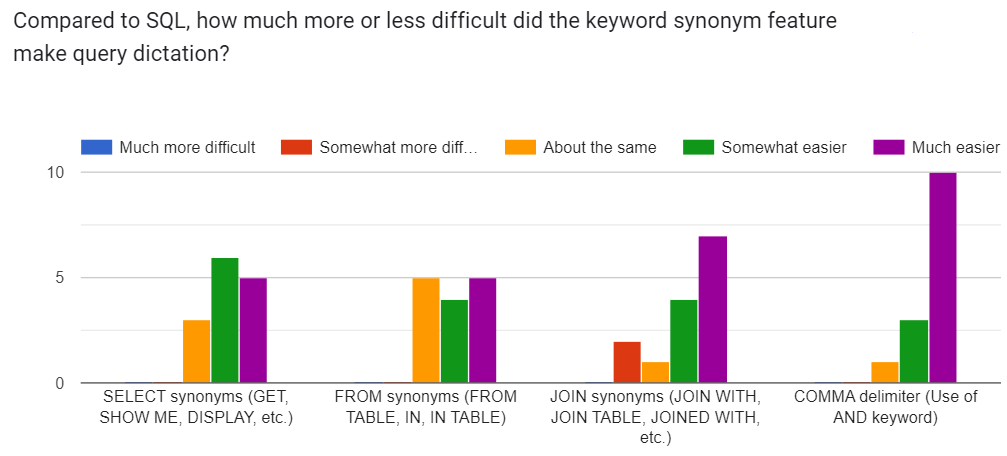
\includegraphics[width=\linewidth]{figures/survey-feedback/10-21-22-kw-synonym.png}
    \caption{Keyword Synonyms}
  \end{subfigure}
  \begin{subfigure}[b]{\linewidth}
    \centering
    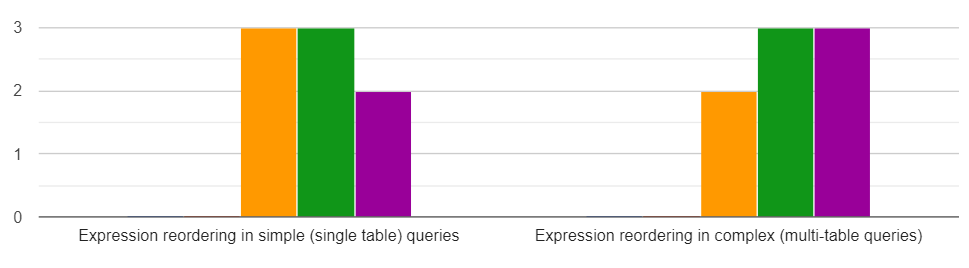
\includegraphics[width=\linewidth]{figures/survey-feedback/10-21-22-expr-ordering.png}
    \caption{Expression Ordering}
  \end{subfigure}
  \begin{subfigure}[b]{\linewidth}
    \centering
    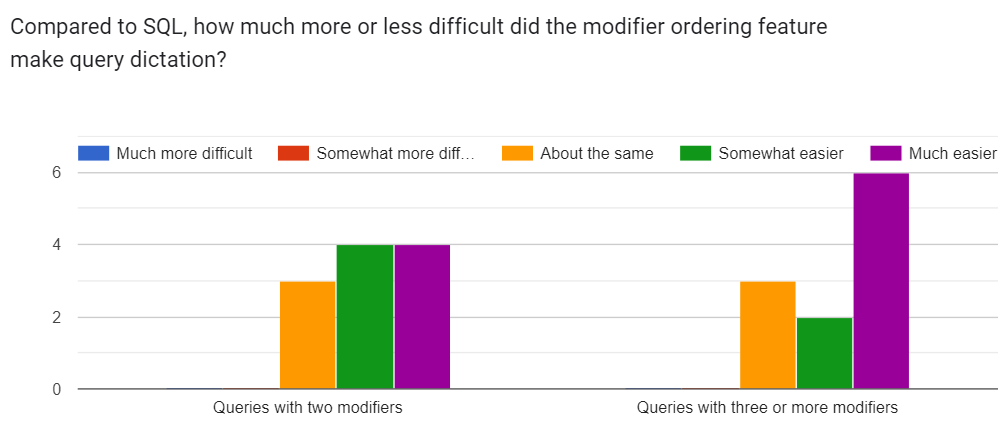
\includegraphics[width=\linewidth]{figures/survey-feedback/10-21-22-modifier-ordering.png}
    \caption{Modifier Ordering}
  \end{subfigure}
  \begin{subfigure}[b]{\linewidth}
    \centering
    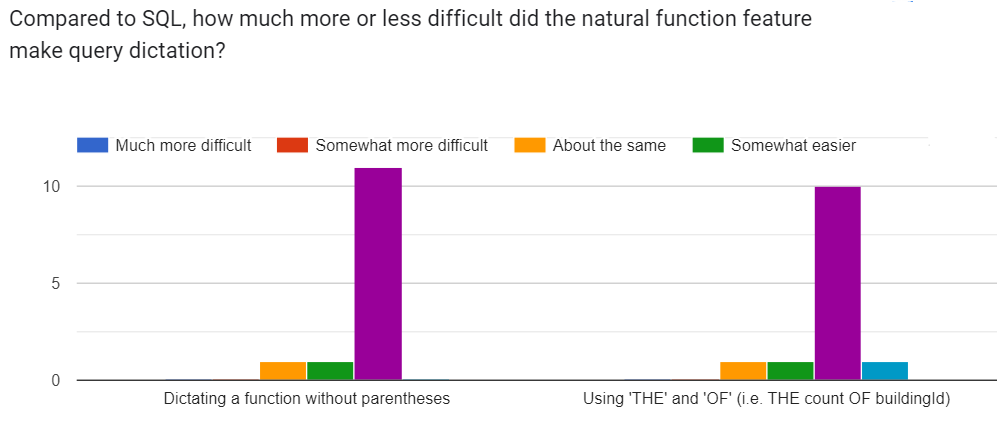
\includegraphics[width=\linewidth]{figures/survey-feedback/10-21-22-nat-func.png}
    \caption{Natural Functions}
  \end{subfigure}
  \begin{subfigure}[b]{\linewidth}
    \centering
    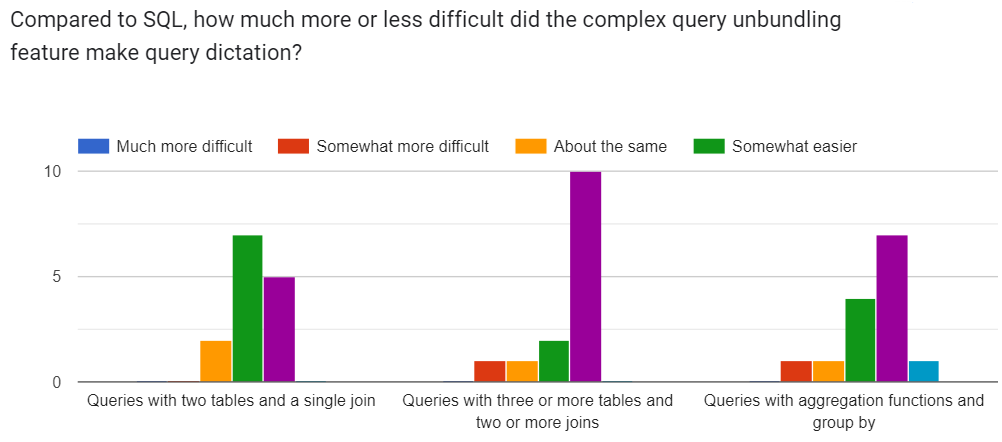
\includegraphics[width=\linewidth]{figures/survey-feedback/10-21-22-unbundling.png}
    \caption{Unbundling}
  \end{subfigure}
  \caption{User Study: Feature Usefulness Survey Results}
  \label{fig:surveyusefulnessgraphs}
\end{figure}

\thematiccoding


\section{Conclusion}


SpeakQL is an ongoing project with the objective of improving the experience of querying arbitrary relational databases using speech-based technology. We used the preliminary work on SpeakQL \cite{Shah2020} as a starting point to develop the SpeakQL dialect, which is an extension of SQL formal grammar to make the language feel more natural for users while retaining SQL's formality and expressive power.

Work on SpeakQL is ongoing including implementation of automatic speech recognition features, application of SpeakQL 1.0 structural and literal determination methods to the more verbose SpeakQL dialect, and integration of user feedback from the ongoing user study. As we continue developing SpeakQL 2.0 toward these objectives, we intend to perform additional user studies to measure the effectiveness of SpeakQL's updates quantitatively and qualitatively based on feedback from its intended user populations. 

Additional research areas related to SpeakQL and the SpeakQL language dialect include the study of mixed initiative user interfaces to enable stateful and incremental query building, error correction and disambiguation through human-computer dialogue, and parser and translation performance optimization to enable near-real-time interaction using more complex grammars such as the SpeakQL dialect.

